\begin{savequote}[75mm]
Some Quote.
\qauthor{Quoteauthor Lastname}
\end{savequote}

%For an example of a full page figure, see Fig.~\ref{fig:myFullPageFigure}.
\chapter{Model-Based Point Cloud Tracking}
\label{Chap:ModelBasedTracking}
\newthought{There's something to be said} for having a good opening line. 

\begin{figure*}[!ht]
  \centering
  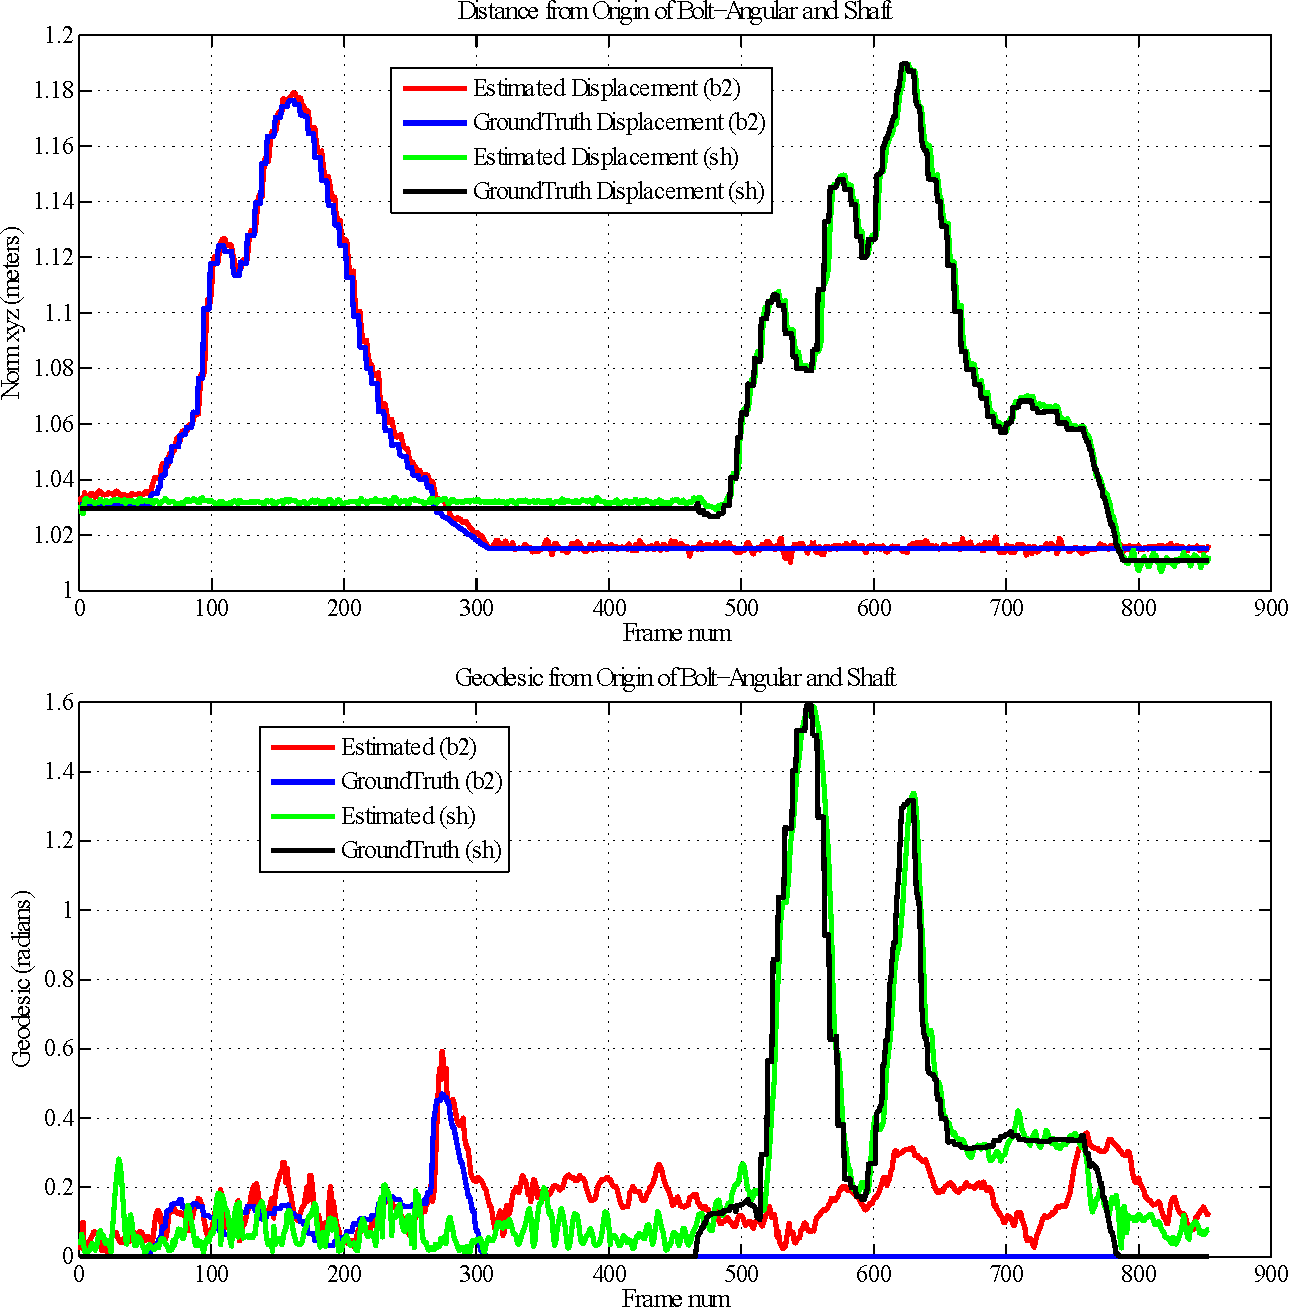
\includegraphics[width=\linewidth]{figures/Tracking/CombinedNoNoise.pdf}
  \caption[Tracked Output vs Ground Truth Artificial Sequence]{Tracked Output vs Ground Truth Artificial Sequence. The top panel shows position in terms of XYZ displacement and the bottom shows rotation in terms of geodesic. The location is generally tracked quite well, while the rotation is noisy due to the rotational symmetry of the two tracked objects (a bolt-angular and shaft).}
  \label{fig:CombinedNoNoise}
\end{figure*}

\begin{figure*}[!ht]
  \centering
  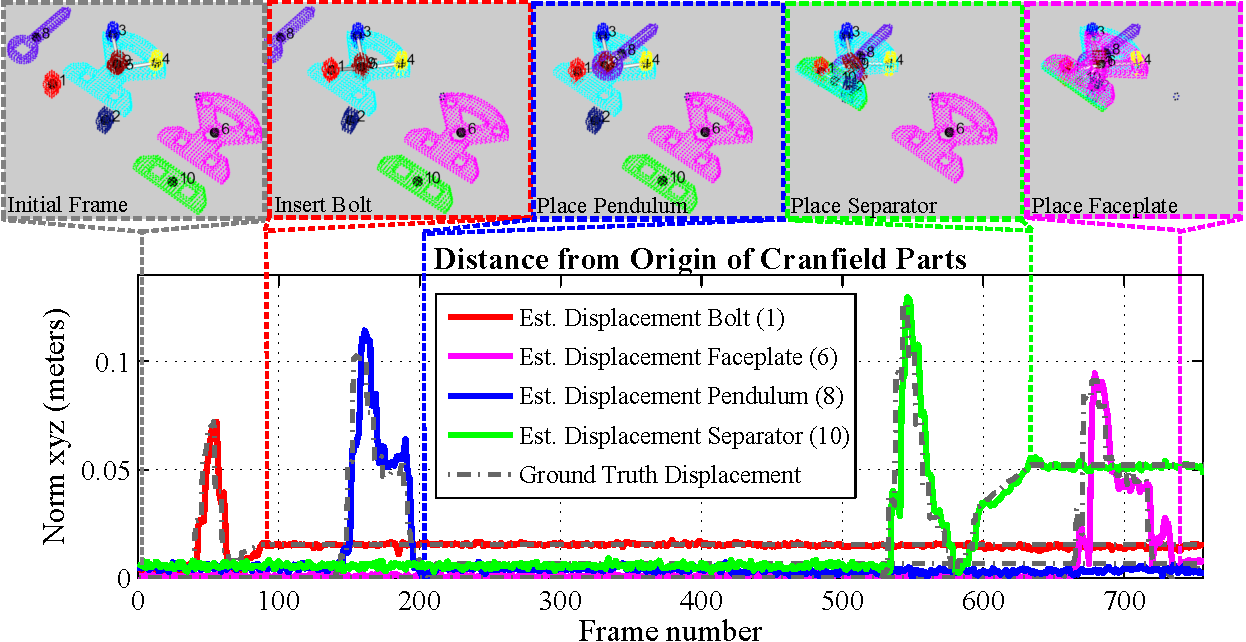
\includegraphics[width=\linewidth]{figures/Tracking/Action_Segmentation.pdf}
  \caption[Segmentation of Actions]{Segmentation of Cranfield Sequence into Keyframes - Tracked objects are monitored for when interactions between them occur, yielding keyframes which correspond to semantically important frames. Results here are shown for an artificial sequence with depth and RGB noise added.}
  \label{fig:ActionSegmentation}
\end{figure*}






